\chapter{Materiais e Métodos}
\label{chap:materiais-e-metodos}

Neste capítulo, são apresentadas as principais tecnologias e ferramentas empregadas ao longo deste 
trabalho, bem como uma descrição detalhada dos algoritmos estudados. A Seção \ref{sec:python} aborda a 
linguagem de programação empregada no desenvolvimento do algoritmo proposto por Marques. A Seção 
\ref{chap:algoritmos-trabalhados} discute os algoritmos que serão comparados ao método desenvolvido pelo 
autor. Por fim, a Seção \ref{cap:projeto_experimento} descreve a metodologia experimental adotada e explica 
como o experimento foi conduzido.

\section{Python}
\label{sec:python}
Python é uma linguagem de programação interpretada de alto nível e que suporta múltiplos paradigmas de 
programação: imperativo, orientado a objetos e funcional. É uma linguagem com tipagem dinâmica e 
gerenciamento automático de memória \cite{pereira2020sistema}.

A linguagem \textit{Python} foi escolhida pela facilidade de criar e manusear uma Inteligência Artificial (IA), que deixa o desenvolvimento mais fluído e de forma mais orgânica \cite{deolhar}.

\section{Algoritmos Trabalhados}
\label{chap:algoritmos-trabalhados}

Neste trabalho, foram analisados e avaliados os algoritmos de Luhn \cite{luhn1957stoical}, \textit{GistSumm} \cite{gistsumm}, o algoritmo de Programação Linear Inteira \cite{oliveira2018sumarizaccao}, um algoritmo de regressão Bayesiana \cite{sodre2019avaliando}, o \textit{ChatGPT} \cite{rudolph2023chatgpt} e um algoritmo criado pelo pesquisador dessa monografia, todos sumarizadores baseados na extração de palavras-chave do texto. 

O algoritmo de Luhn é um dos trabalhos mais importantes na área de PLN, em Sumarização de Documentos \cite{luhn1957stoical}, é um algoritmo clássico que serviu como base para muitos algoritmos, seu método de extração é baseado na extração de palavras-chave.

Os algoritmos citados anteriormente são embasados no algoritmo de Luhn, mas desenvolvidos a partir de abordagens distintas, como técnicas de regressão, inferências Bayesianas, além de mostrarem que utilizando a sentença principal do texto é mais eficiente quando se trata de gerar resumos com as ideias principais de um texto \cite{salvino2019analise}.

Os algoritmos estudados são mais utilizados para sumarizar textos que não são monografias, artigos, pesquisas cientificas e outros dentro dessa área.

Além de analisar os principais desafios da área de sumarização automática de textos, o objetivo deste trabalho é a criação de um algoritmo que se destine especificamente à produção de resumos de textos acadêmicos, como monografias, artigos e pesquisas. Dessa forma, busca-se contribuir com a comunidade científica, fornecendo uma ferramenta que facilite a criação literária e pesquisa, ao mesmo tempo em que se avança no conhecimento sobre a área de sumarização automática de textos.

\section{Projeto do Experimento}
\label{cap:projeto_experimento}

Esta seção, descreve o planejamento e execução do experimento de comparação dos algoritmos, com o objetivo de determinar qual deles melhor atende às expectativas do usuário.

\subsection{Instrumentação}
\label{chap:instrumentacao}

A instrumentação dos experimentos é dividida em hardware e software. Será utilizado um computador equipado com um processador Intel Core i5-10500H (10ª geração) \textit{Quad Core} para executar um conjunto de códigos-fonte em \textit{Python} 3.10, que implementam os algoritmos a serem avaliados.

\subsection{Etapas do Experimento}
\label{chap:experimento}

O experimento é composto por três etapas, conforme ilustrado na Figura \ref{fig:projeto-experimento}:

\begin{figure}[!h]
\centering
    \caption{Etapas do Experimento}
    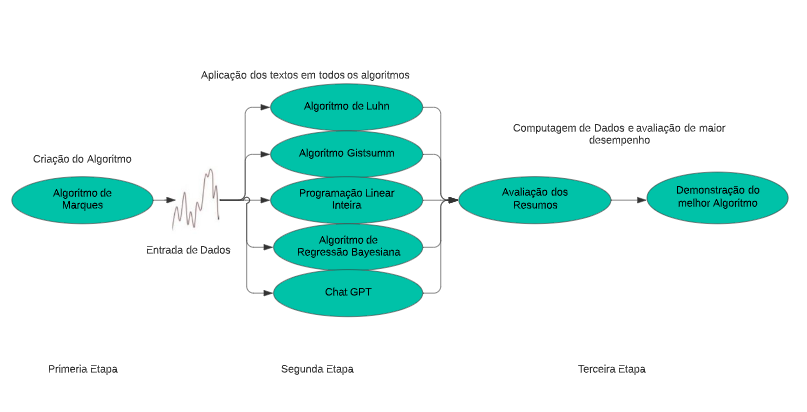
\includegraphics[width=\textwidth]{figuras/design-experimento.png}
    \label{fig:projeto-experimento}
    \Fonte{Autoria própria.}
\end{figure}

A avaliação de desempenho dos algoritmos foi realizada com base em métricas como taxa de coerência, taxa de coesão, precisão e tempo de processamento. Essas métricas são amplamente utilizadas na literatura para avaliar a qualidade dos resumos gerados por algoritmos de sumarização automática de texto \cite{pandian2021performance}. A seguir, serão apresentadas as definições e explicações detalhadas de cada métrica utilizada.
\begin{itemize}
    \item Coerência: A taxa de coerência avalia a lógica e a clareza da     estrutura do resumo gerado. Um resumo coerente deve apresentar as informações de maneira lógica, com uma sequência que faça sentido e     seja fácil de seguir pelo leitor. A coerência pode variar de 0 a 1, sendo que valores mais próximos de 1 indicam maior coerência no resumo gerado.

    \item Coesão: A taxa de coesão mede o grau de conexão entre as ideias presentes no resumo gerado. Um resumo coeso deve apresentar ideias relacionadas de maneira integrada e harmoniosa, sem lacunas ou informações desconexas. A coesão também pode variar de 0 a 1, sendo que valores mais próximos de 1 indicam maior coesão no resumo gerado.

    \item Precisão: A precisão avalia a capacidade do algoritmo em selecionar as informações mais relevantes do texto original para 
    compor o resumo. Um resumo preciso deve conter as informações 
    essenciais e mais importantes do texto original, sem incluir 
    informações desnecessárias ou irrelevantes. A precisão pode variar 
    de 0 a 1, sendo que valores mais próximos de 1 indicam maior 
    precisão na seleção de informações relevantes para o resumo.

    \item Tempo de processamento: O tempo de processamento é uma medida 
    do tempo necessário para que o algoritmo processe o texto original e gere o resumo correspondente. Essa métrica é importante para avaliar a eficiência dos algoritmos em termos de rapidez e capacidade de processar grandes volumes de dados. O tempo de processamento é geralmente expresso em segundos, sendo que menores valores indicam um algoritmo mais rápido e eficiente.
\end{itemize}

A análise dessas métricas, fundamentada em estudos prévios e na literatura científica sobre sumarização automática, possibilita uma compreensão aprofundada do desempenho dos algoritmos de sumarização automática. Essa análise fornece informações valiosas para a seleção do algoritmo mais adequado, levando em consideração as necessidades específicas dos usuários.

A Etapa 1 envolve a criação do algoritmo de Marques. Na Etapa 2, o objetivo é realizar a sumarização automática de um artigo sobre a pandemia da COVID-19 e as mudanças no estilo de vida dos brasileiros adultos (\cite{MALTA2020}). O texto que servirá de base para a geração dos resumos está disponível no Anexo \ref{chap:texto_covid} e será processado através de seis algoritmos distintos. Por fim, na Etapa 3, os resumos serão avaliados por um grupo de avaliadores, que julgarão a qualidade dos resumos gerados por cada algoritmo, a fim de determinar o desempenho de cada um deles.

O cenário considerado para os experimentos envolve a simulação de resumos em uma máquina virtual com capacidade de processamento de um Intel Core i5 10500H (10ª geração) – 12 MB de cache, 6 núcleos e 12 \textit{threads} – com frequência de 2.50 GHz até 4.50 GHz e 16 GB de memória RAM. A análise das sumarizações obtidas será realizada dentro de um contexto educacional.

\subsubsection{Etapa 1: Criação do Algoritmo de Marques}
\label{chap:primeira-etapa}

A primeira etapa consiste na criação do algoritmo de Marques, que começa criando uma matriz do texto, dividindo-o em sentenças e, em seguida, em palavras. Então, identifica palavras com função sintática, mas sem relevância semântica, como "ou", "e", "para", e as remove da matriz. Isso é feito porque essas palavras são frequentes e acabariam recebendo importância indevida, dificultando a análise textual. Pontuações também são removidas, pois o algoritmo as trata como palavras, o que atrapalha a sumarização.

Após a limpeza do texto, o algoritmo cria uma distribuição de frequência para a matriz de palavras, identificando as mais importantes. Com base nessa distribuição, o algoritmo seleciona as palavras mais comuns, de acordo com um valor pré-determinado, para posteriormente classificá-las como relevantes ou não no resumo final.

\subsubsection{Etapa 2: Sumarização Automática}
\label{chap:segunda-etapa}

A segunda etapa, consiste em realizar a sumarização automática usando os algoritmos de Luhn, \textit{Gistsumm}, PLI \cite{oliveira2018sumarizaccao}, regressão Bayesiana, \textit{ChatGPT} e o algoritmo de Marques.

Foram realizados testes nas configurações dos parâmetros comuns modificáveis nos algoritmos, isto é, na quantidade de sentenças importantes, a fim de equipará-los para a etapa seguinte. Dessa forma, neste experimento foi utilizado o parâmetro de \textbf{cinco (5) sentenças importantes}.

Segundo \citeonline{rino2003sumarizaccao}, para gerar um resumo eficiente, deve-se extrair entre 20 a 50\% do texto e atingir uma taxa de compressão de 80\%. Neste trabalho, seguimos essa orientação ao avaliar os algoritmos de sumarização automática.

Considerando os parâmetros mencionados, o texto utilizado no resumo seguiu uma taxa de compressão de aproximadamente 40\% para cada algoritmo. O algoritmo de Marques, por exemplo, selecionou as cinco sentenças mais importantes do texto original, que representam uma porcentagem significativa das informações relevantes. Essas cinco sentenças foram determinadas com base na frequência das palavras e na relevância das sentenças no contexto do texto.

As cinco sentenças importantes servem como um critério para avaliar a qualidade dos resumos gerados pelos algoritmos de sumarização automática. A escolha dessas sentenças permite obter um resumo conciso e informativo, mantendo a essência do texto original e assegurando que o leitor compreenda os principais pontos abordados. Esse critério contribui para a eficiência dos resumos gerados e auxilia na comparação dos algoritmos em relação à sua capacidade de extrair informações relevantes e concisas do texto original \cite{oliveira2022composiccao}.

\subsubsection{Etapa 3: Avaliação dos Resumos}
\label{chap:terceira-etapa}

Para avaliar a qualidade e coesão dos resumos gerados na segunda etapa, foram coletadas 49 respostas 
de indivíduos com diferentes graus de instrução acadêmica que responderam a questionários aleatórios. Essas pessoas avaliaram os resumos resultantes da inserção do artigo de \citeonline{MALTA2020} distribuídos entre 6 resumos e 5 questionários, comparando cada algoritmo mencionado na segunda etapa com o algoritmo de Marques.

Os avaliadores julgaram qual texto apresentava maior coesão e coerência, sem saber quais algoritmos foram utilizados. Em todos os casos, o texto 1 representa o resumo proveniente do algoritmo de Marques, enquanto o texto 2 em cada questionário representa os algoritmos comparados: Luhn, \textit{Gistsumm}, PLI \cite{oliveira2018sumarizaccao}, regressão Bayesiana e \textit{ChatGPT}.

Os questionários foram enviados por meio de formulários no \textit{Google Docs}, conforme modelo apresentado no Apêndice \ref{ap:Forms}.

\subsection{Amostragem e Seleção dos Participantes}
\label{subsec:amostragem}

A escolha dos participantes para a avaliação dos algoritmos de sumarização automática neste trabalho foi feita através de uma amostragem por conveniência. A amostragem por conveniência é uma técnica não probabilística que seleciona os participantes com base na disponibilidade e na facilidade de acesso \cite{neuman2006workbook}.

Os questionários foram preenchidos pelos participantes após a divulgação dos formulários pelas redes sociais do autor e do orientador. Esse método de seleção permitiu alcançar um grupo diversificado de participantes, embora não seja uma amostra totalmente representativa da população em geral.

É importante mencionar que a amostragem por conveniência pode ter sido influenciada pelo efeito \textit{snowball} \cite{goodman1961snowball}. O efeito \textit{snowball} ocorre quando os participantes iniciais compartilham o questionário com seus contatos, que por sua vez compartilham com seus próprios contatos, aumentando o alcance da pesquisa. Esse efeito pode introduzir viés na amostra, uma vez que as pessoas que participam da pesquisa tendem a ter características semelhantes ou estarem 
relacionadas de alguma forma.

Apesar dessas limitações, a amostragem por conveniência e o possível efeito \textit{snowball} permitiram obter um número suficiente de respostas para a avaliação dos algoritmos de sumarização automática, fornecendo informações valiosas sobre o desempenho dos algoritmos em relação às métricas estabelecidas.

Após a coleta das respostas, os resultados foram processados e analisados com base em métricas específicas de qualidade de sumarização, como precisão, coerência e coesão, além do tempo de processamento. Essa análise permitiu determinar qual algoritmo apresentou melhor desempenho na geração de resumos coerentes e coesos. Os algoritmos utilizados na comparação e seus respectivos métodos de sumarização serão detalhados no capítulo \ref{cap:algoritmos}.